\documentclass[hidelinks,a4paper,10pt, nofootinbib]{article}
\usepackage{geometry}
\usepackage[spanish, es-tabla]{babel} %es-tabla es para que ponga Tabla en vez de Cuadro en el caption
\usepackage[utf8]{inputenc}
\usepackage[T1]{fontenc}
\usepackage{xspace}
\usepackage{xargs}
\usepackage{fancyhdr}
\usepackage{lastpage}
\usepackage{caratula}
\usepackage{enumitem} %Permite modificar los margenes de lsa listas
\usepackage[bottom]{footmisc}
\usepackage{amsmath}
\usepackage{amssymb}
\usepackage{algorithm}
\usepackage[noend]{algpseudocode}
\usepackage{array}
\usepackage{xcolor,colortbl}
\usepackage{amsthm}
\usepackage{listings}
\usepackage{soul}
\usepackage{graphicx}
\usepackage{sidecap}
\usepackage{amsmath}
\usepackage{wrapfig}
\usepackage{caption}
\usepackage{mathpazo}

\setlength{\parindent}{4em}
\setlength{\parskip}{1em}

%Formato de los links
\usepackage{hyperref}
\hypersetup{
  colorlinks   = true, %Colours links instead of ugly boxes
  urlcolor     = blue, %Colour for external hyperlinks
  linkcolor    = blue, %Colour of internal links
  citecolor   = red %Colour of citations
}

\usepackage{comment}
\captionsetup[table]{labelsep=space}


\setlength{\parindent}{4em}
\setlength{\parskip}{0.5em}


%%fancyhdr
\pagestyle{fancy}
\thispagestyle{fancy}
\addtolength{\headheight}{1pt}
\lhead{Ingeniería del Software I+II: TP2}
\rhead{$2º$ cuatrimestre de 2016}
\cfoot{\thepage\ / \pageref{LastPage}}
\renewcommand{\footrulewidth}{0.4pt}
\renewcommand{\labelitemi}{$\bullet$}

%%caratula
\materia{Ingeniería del Software I+II}
\titulo{Trabajo Práctico Número 2}
\subtitulo{ReciBarFiesta}
\grupo{Grupo 7}
\integrante{Ciruelos Rodríguez, Gonzalo}{063/14}{gonzalo.ciruelos@gmail.com}
\integrante{Costa, Manuel José Joaquín}{035/14}{manucos94@gmail.com}
\integrante{Gatti, Mathias Nicolás}{477/14}{mathigatti@gmail.com}
\integrante{Maddonni, Axel Ezequiel}{200/14}{axel.maddonni@gmail.com}
\integrante{Thibeault, Gabriel}{114/13}{gabriel.eric.thibeault@gmail.com}

% \fecha{24 de Junio de 2016}
\begin{document}

\maketitle

\tableofcontents
\newpage

\section{Introducción}
El trabajo práctico se basa en el desarrollo de una aplicación llamada ReciBarFiesta. El trabajo consiste de dos entregas, la primera concierne a la planificación y la segunda a la arquitectura. La parte de planificación consiste en:
\begin{itemize}  
  \item un plan del proyecto,
  \item una lista de casos de uso,
  \item un análisis de riesgos.
\end{itemize}
En este trabajo presentamos toda esa información (en un orden que nos pareció más sensato) y justificamos nuestras decisiones.

\newpage

\section{Casos de uso}
% Please add the following required packages to your document preamble:
% \usepackage[table,xcdraw]{xcolor}
% If you use beamer only pass "xcolor=table" option, i.e. \documentclass[xcolor=table]{beamer}
\begin{table}[H]
\centering
\begin{tabular}{|l|l|c|}
\hline
\rowcolor[HTML]{CBCEFB} 
\multicolumn{1}{|c|}{\cellcolor[HTML]{CBCEFB}\textbf{Código}} & \multicolumn{1}{c|}{\cellcolor[HTML]{CBCEFB}\textbf{Caso de uso}} & \textbf{Horas Hombre} \\ \hline
CU01                                                          & Incluyendo un evento cultural                                     & 30                    \\ \hline
CU02                                                          & Eliminando un evento cultural                                     & 8                     \\ \hline
CU03                                                          & Buscando evento                                                   & 56                    \\ \hline
CU04                                                          & Rankeando evento                                                  & 60                    \\ \hline
CU05                                                          & Logueándose                                                       & 59                    \\ \hline
CU06                                                          & Compartiendo información en redes sociales                        & 8                     \\ \hline
CU07                                                          & Editando un evento cultural                                       & 8                     \\ \hline
CU08                                                          & Registrándose                                                     & 20                    \\ \hline
CU09                                                          & Verificando contenido inapropiado automáticamente                 & 48                    \\ \hline
CU10                                                          & Verificando contenido inapropiado manualmente                     & 8                     \\ \hline
CU11                                                          & Reservando hoteles                                                & 56                    \\ \hline
CU12                                                          & Reservando vuelos                                                 & 48                    \\ \hline
CU13                                                          & Enviando publicidad                                               & 20                    \\ \hline
CU14                                                          & Visualizando caminos                                              & 48                    \\ \hline
CU15                                                          & Realizando reserva                                                & 56                    \\ \hline
CU16                                                          & Filtrando resultados                                              & 20                    \\ \hline
CU17                                                          & Obteniendo estadísticas sobre los usuarios                        & 32                    \\ \hline
CU18                                                          & Combinando eventos                                                & 32                    \\ \hline
\end{tabular}
\caption{Casos de uso}
\label{tab:cu}
\end{table}

\subsection{Diagrama de Casos de uso}

\begin{figure}[H]
 \centering
  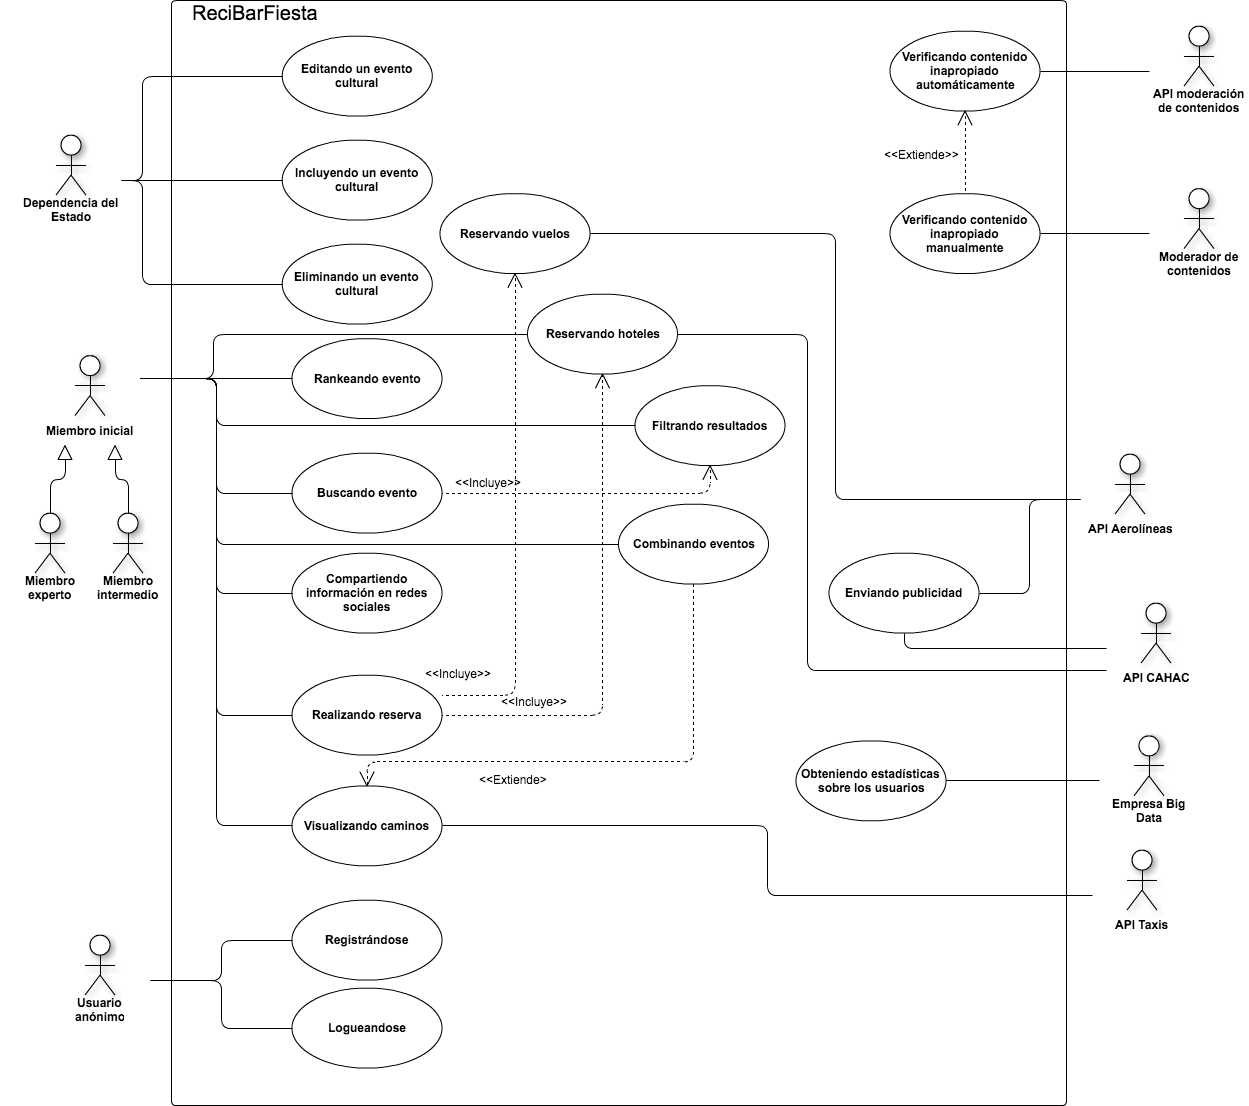
\includegraphics[width=\textwidth]{diagramas/casosDeUso.png}
  \caption{Diagrama de Casos de Uso de ReciBarFiesta}
  \label{fig:cu}
\end{figure}

\subsection{Descripción de los Casos de uso}
\begin{enumerate}
  \item \textbf{Incluyendo un evento cultural:} se refiere a la funcionalidad para agregar nuevos eventos, como recitales, charlas, festivales, etc. Solo lo pueden hacer usuarios autorizados (inicialmente solo miembros de dependencias del Estado).
  \item \textbf{Eliminando un evento cultural:} se refiere a la funcionalidad por la cual una dependencia del Estado puede eliminar un evento cultural previamente creado.
  \item \textbf{Editando un evento cultural:} se refiere a la funcionalidad por la cual una dependencia del Estado puede modificar los datos de un evento cultural previamente creado.
  \item \textbf{Rankeando evento:} se refiere a la funcionalidad que le permite a un miembro identificado de la comunidad calificar un evento en distintas categorías como, por ejemplo, ``Organización'', “Calidad” y “Ubicación”. Solo usuarios identificados podrán realizar esta acción, y se ponderará la calificación de acuerdo a la categoría del usuario (inicial, intermedio o experto).
  \item \textbf{Buscando evento:} se refiere a la funcionalidad por la cual los usuarios de la aplicación buscarán eventos, pudiendo filtrar los resultados por una serie de criterios (por ejemplo: fecha, temática, ubicación, etc) usando el caso de uso ``Filtrando resultados'' (CU16).
  %%%
  %%% ACA VA UNA TABLA
  %%%
  \item \textbf{Compartiendo información en redes sociales:} se refiere a la funcionalidad por la cual los miembros de la comunidad podrán compartir los diferentes eventos disponibles en la aplicación en diferentes redes sociales como Facebook o Twitter, de manera que otras personas que no necesariamente tienen la aplicación puedan conocer su existencia.
  \item \textbf{Logueandose:} se refiere a la funcionalidad por la cual los usuarios anónimos con una cuenta previamente creada podrán identificarse con el sistema, lo cual les habilitará a tener información personalizada (por ejemplo, según el barrio en el que viven), valorar eventos, y poder realizar reservas de vuelos y hoteles.
  \item \textbf{Registrándose:} se refiere a la funcionalidad a través de la cual los usuarios anónimos pueden crearse una cuenta en el sistema, para eventualmente poder identificarse y aprovechar los privilegios que esto acarrea.
  \item \textbf{Verificando contenido inapropiado automatizado:} se refiere a la funcionalidad con la que el sistema utiliza la API de moderación de contenidos. La misma pone puntajes de 1 (contenido inapropiado), 2 (contenido dudoso, proceder a verificación manual) o 3 (contenido seguro)
  \item \textbf{Verificando contenido inapropiado manualmente:} se refiere a la funcionalidad para que un moderador pueda determinar si un determinado contenido es apropiado o no. Este caso de uso solo se activa para aquellos contenidos que son calificados con 2 por CU9.
  \item \textbf{Enviando Publicidad:} se refiere a la funcionalidad que le permite a los sponsors económicos de la aplicación enviar su material publicitario para ser mostrado por la página.
  \item \textbf{Visualizando Caminos:} se refiere a la funcionalidad que permite a los usuarios visualizar el o los caminos (en caso de que se hayan seleccionado múltiples eventos) desde su posición actual hasta cada evento. Se ofrecen diferentes tipos de rutas: caminando, en auto particular, en taxi (usando la aplicación del gobierno de la Ciudad), y en transporte público. Eventualmente pueden combinarse eventos (CU18).
  \item \textbf{Reservando Hoteles:} se refiere a la funcionalidad por la cual la API del sistema de la Cámara de Hoteles y Afines de la Ciudad (CAHAC) podrá registrar reservas de hoteles efectuadas por usuarios de la aplicación.
  \item \textbf{Reservando Vuelos:} se refiere a la funcionalidad por la cual la API del sistema de Aerolíneas Argentinas podrá registrar reservas de vuelos efectuadas por usuarios de la aplicación.
  \item  \textbf{Obteniendo estadísticas sobre los usuarios:} se refiere a la API desarrollada para que las empresas de Big Data puedan obtener los datos estadísticos sobre los usuarios.
  \item  \textbf{Filtrando resultados:} se refiere a la funcionalidad que le permite a los usuarios de la aplicación filtrar listas de eventos según diversos criterios a determinar.
  \item  \textbf{Realizando Reserva:} se refiere a la funcionalidad por la cual los miembros de la comunidad podrán seleccionar y reservar vuelos/hoteles para participar de eventos publicados en la aplicación utilizando los servicios provistos por Aerolíneas Argentinas, para vuelos, y de la Cámara de Hoteles y Afines de la Ciudad, para alojamientos .
  %%%
  %%% ACA VA UNA TABLA
  %%%
  \item \textbf{Combinando eventos:}  se refiere a la funcionalidad que extiende al caso CU10, permitiendo combinar eventos de forma tal que se obtenga el mejor camino que pasa por todas las ubicaciones.
\end{enumerate}


\newpage

\section{Riesgos}
\paragraph{Riesgo 1}
\begin{itemize}  
  \item \textbf{Descripción:} Dado que se pueden dar problemas de conexión y se requiere que todos los días extraigan los datos (por  limitaciones de espacio) se podría llegar a fallar en entregar los datos pedidos a las compañías de big data.
  \item \textbf{Probabilidad:} Baja
  \item \textbf{Impacto:} Medio
  \item \textbf{Exposición:} Baja
  \item \textbf{Mitigación:} Tener el espacio necesario para almacenar, como mínimo, el doble de la información que esperamos almacenar en promedio.
  \item \textbf{Plan de contingencia:} En caso de que el servicio de big data este caído por varios días y no queramos perder información, se debería hacer backup manual de los datos antes de que sean sobreescritos.
\end{itemize}

\paragraph{Riesgo 2}
\begin{itemize}
  \item \textbf{Descripción:} No tener la integración con Aerolíneas y CAHAC hecha para el 2017.
  \item \textbf{Probabilidad:} Media
  \item \textbf{Impacto:} Alto
  \item \textbf{Exposición:} Alta
  \item \textbf{Mitigación:} Completar la integración en las primeras dos iteraciones del desarrollo. Asignar a los mejores programadores y más recursos a realizar esta tarea.
  \item \textbf{Plan de contingencia:} En caso que muchos eventos imprevistos suceden y no se llegue a tiempo, se podría pedir una extensión a Aerolíneas con la suficiente anticipación. Además, se podría hacer que el equipo abandone el desarrollo de otras funcionalidades y se aboque en su totalidad a finalizar la integración.
\end{itemize}

\paragraph{Riesgo 3}
\begin{itemize}
  \item \textbf{Descripción:} Incapacidad del sistema de moderación principal para procesar los pedidos en tiempo real (Tanto de congestión como por caída del sistema).
  \item \textbf{Probabilidad:} Alta (Depende fuertemente del sistema).
  \item \textbf{Impacto:} Baja
  \item \textbf{Exposición:} Media
  \item \textbf{Mitigación:} Realizar estudios para tener una excelente aproximación de tráfico, de tal manera de poder comunicarlo a la empresa que provee el servicio. Tener un servicio secundario, de tal manera que si el primario se cae o funciona mal, podamos usarlo.
  \item \textbf{Plan de contingencia:} En caso que todo falle y no podamos analizar comentarios en tiempo real, podemos almacenarlos en una cola y para que sean analizados más adelante cuando todo vuelva a la normalidad. En caso que el sistema tarde mucho en volver a la normalidad, perderemos comentarios.
\end{itemize}

\paragraph{Riesgo 4}
\begin{itemize}
  \item \textbf{Descripción:} Perder la conexión a internet.
  \item \textbf{Probabilidad:} Baja
  \item \textbf{Impacto:} Alto
  \item \textbf{Exposición:} Media
  \item \textbf{Mitigación:} Tener una conexión secundaria (o más de una) de tal manera que si se cae, podamos usar esa.
  \item \textbf{Plan de contingencia:} Deberíamos tener un sistema rotatorio de on-calls, de tal manera que si se cae internet, en cualquier momento se le avise al on-call y este se ocupe de trasladar el servicio a una nueva conexión.
\end{itemize}

\paragraph{Riesgo 5}
\begin{itemize}
  \item \textbf{Descripción:} Filtración de datos privados
  \item \textbf{Probabilidad:} Baja
  \item \textbf{Impacto:} Alto
  \item \textbf{Exposición:} Media
  \item \textbf{Mitigación:} Diseñar un sistema de detección de intrusiones. Enviar datos al servicio de big data de forma encriptada y des-asociada del nombre del usuario.
  \item \textbf{Plan de contingencia:} Almacenar los datos personales de las cuentas de las personas de forma encriptada, de tal manera que si se filtran no sean legibles.
\end{itemize}

\paragraph{Riesgo 6}
\begin{itemize}
  \item \textbf{Descripción:} Usuarios creados con la intención de manipular la valoración de los eventos
  \item \textbf{Probabilidad:} Alta
  \item \textbf{Impacto:} Bajo
  \item \textbf{Exposición:} Media
  \item \textbf{Mitigación:} Pedir datos personales a la hora de crear la cuenta (Por ejemplo DNI o CUIT).
  \item \textbf{Plan de contingencia:} Diseñar un sistema que detecte que un evento está recibiendo muchas valoraciones y avise al on-call para que realice una revisión manual de la situación.
\end{itemize}

\paragraph{Riesgo 7}
\begin{itemize}
  \item \textbf{Descripción:} Renuncia de personal clave del equipo de desarrollo.
  \item \textbf{Probabilidad:} Baja
  \item \textbf{Impacto:} Medio
  \item \textbf{Exposición:} Baja
  \item \textbf{Mitigación:} Distribuir el trabajo de manera de que nadie esté demasiado sobrecargado y todos conozcan todo lo que se hace.
  \item \textbf{Plan de contingencia:} En caso de renuncias, reorganizar el equipo de tal manera que el programador que más conozco el trabajo del programador que renunció retome sus tareas.
\end{itemize}

\paragraph{Riesgo 8}
\begin{itemize}
  \item \textbf{Descripción:} Que el tráfico promedio de usuarios sea más del previsto y los sistemas internos estén continuamente sobrecargados.
  \item \textbf{Probabilidad:} Baja (Suponiendo una buena estimación inicial)
  \item \textbf{Impacto:} Alto
  \item \textbf{Exposición:} Media
  \item \textbf{Mitigación:} Hacer estimaciones lo mejor posibles.
  \item \textbf{Plan de contingencia:} Diseñar un balanceador de cargas y usarlo. Tener varias instancias del servidor corriendo en paralelo y totalmente replicadas.
\end{itemize}

\paragraph{Riesgo 9}
\begin{itemize}
  \item \textbf{Descripción:} Si la cantidad de ventas de hoteles y boletos de avión no fuera la suficiente, Aerolíneas podría retirar su inversión.
  \item \textbf{Probabilidad:} Baja (Muy difícil de estimar).
  \item \textbf{Impacto:} Medio
  \item \textbf{Exposición:} Media
  \item \textbf{Mitigación:} Hacer que la integración con Aerolíneas sea impecable. Diseñar publicidades llamativas pero poco invasivas.
  \item \textbf{Plan de contingencia:} Cuando la aplicación esté funcionando, invertir tempranamente en hardware y ahorrar dinero para poder hacer una inversión grande en caso que Aerolíneas Argentinas retire la suya.
\end{itemize}
\newpage

\setlist[itemize]{leftmargin=2.5cm}
\section{Plan de Proyecto}
\subsection{WBS}

\begin{figure}[H]
 \centering
  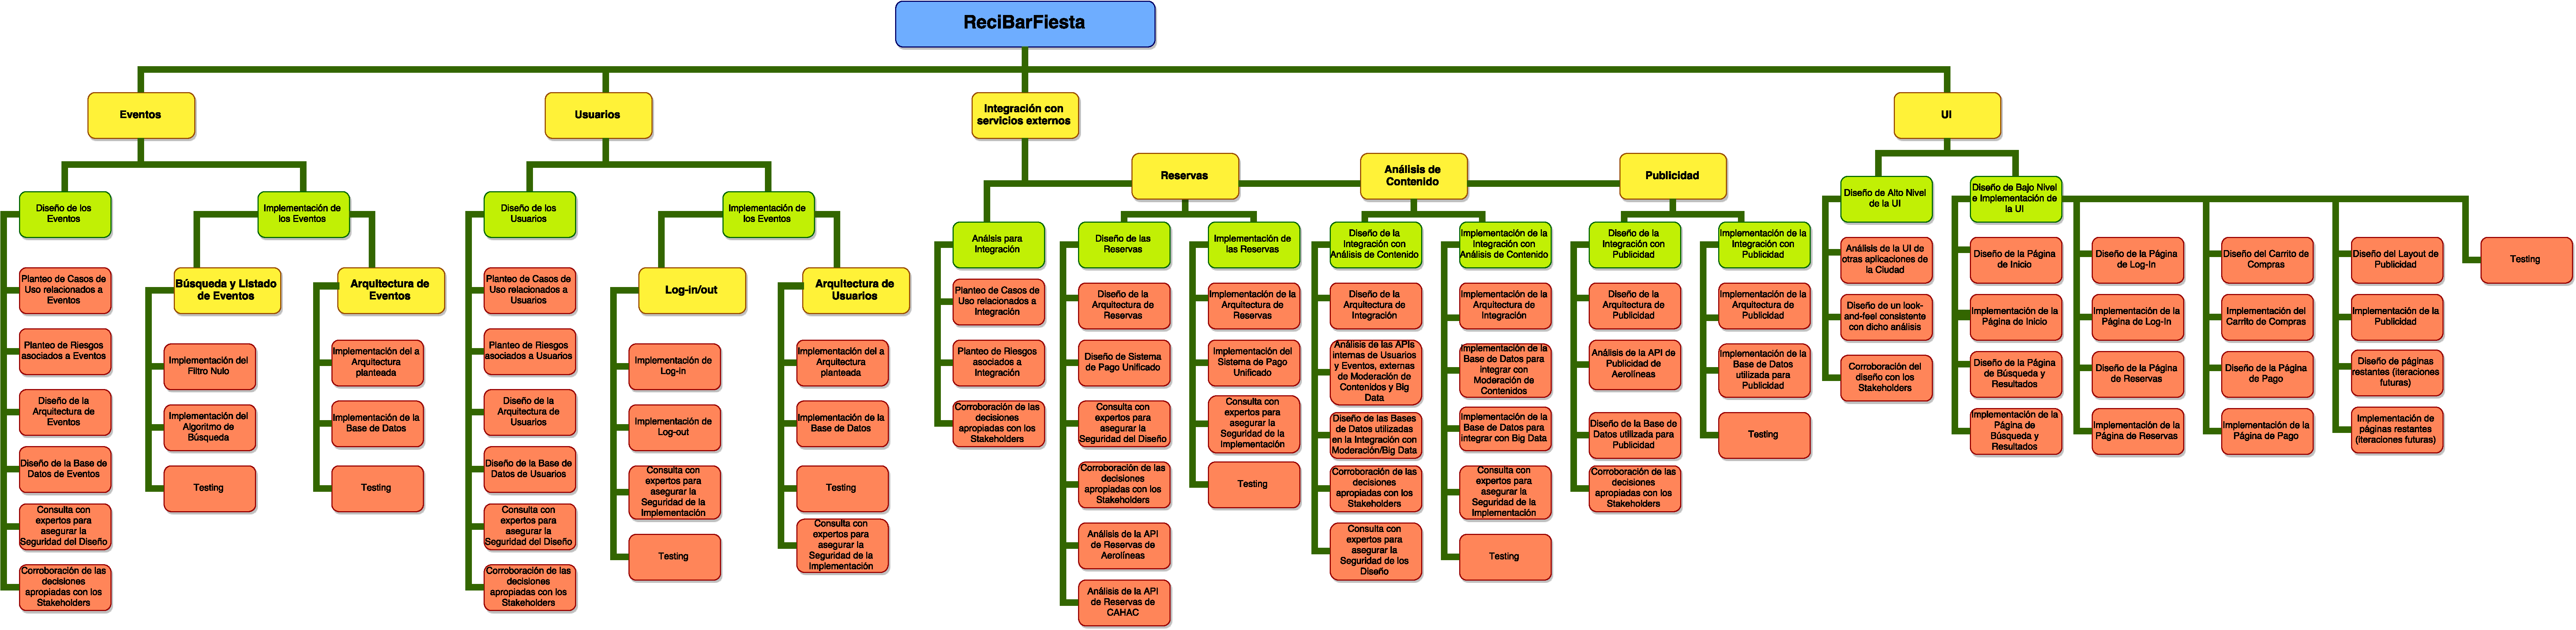
\includegraphics[width=\textwidth]{diagramas/WBS.pdf}
  \caption{WBS}
  \label{fig:wbs}
\end{figure}

En la figura \ref{fig:wbs} puede observarse el diagrama del WBS. Los nodos amarillos representan productos; los verdes, procesos; los rojos, tareas, independientemente de que sean productos o procesos.
Cabe realizar algunas aclaraciones respecto del diagrama. El diseño de la arquitectura del sistema se realizará para la próxima entrega; algunas de las subdivisiones en tareas se basan en dicho diseño, por lo que se observan múltiples instancias de tareas placeholder de la forma “Implementación de la Arquitectura de X”. Tras realizar dicha arquitectura, éstas se deberían separar en las tareas más granulares a realizar.
Es decir, en el WBS nos limitamos a presentar una visión de alto nivel de las subdivisiones del proyecto, que serían refinadas al proceder con el proceso de diseño. El enfoque más específico se reserva para los productos, procesos y tareas correspondientes a los Casos de Uso que fueron designados a la primera iteración.

\subsection{Primera iteración}
Para reflejar el orden en que llevaremos a cabo la primera iteración realizamos un diagrama de Gantt (figura \ref{fig:gantt}) el cual modela, entre otras cosas, las dependencias, duraciones y fechas de inicio de cada tarea; sirviendonos de guía al llevar a cabo el proyecto y para identificar puntos delicados en nuestro plan, utilizando criterios como el de camino crítico. 

\begin{figure}[H]
 \centering
  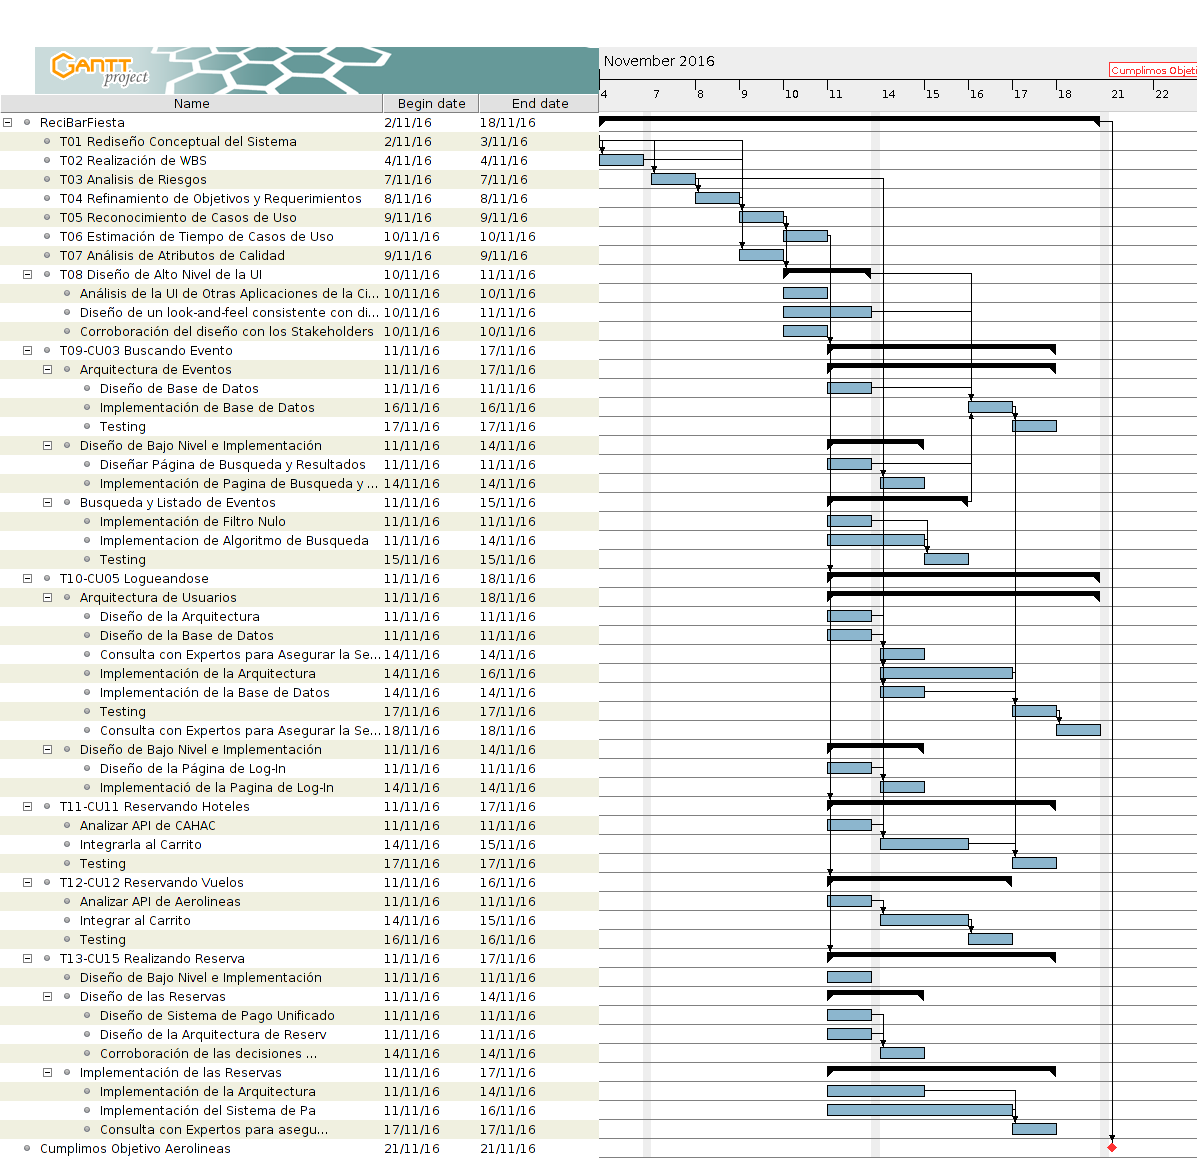
\includegraphics[width=\textwidth]{diagramas/gantt.png}
  \caption{Diagrama de Gantt para la primer iteración del proyecto}
  \label{fig:gantt}
\end{figure}

\subsubsection{Justificación}
Como vimos antes, deberíamos priorizar tener la integración con Aerolíneas Argentinas terminada lo más rápido posible, de tal manera de mitigar el riesgo de no tenerla terminada para 2017. Nótese que es el único riesgo que encontramos al cual tenemos exposición alta. De esta manera, pusimos en la primera iteración todo lo relacionado con la compra de pasajes de avión y reserva de hoteles. Esta es la parte más delicada de la integración. El cumplimiento de este objetivo se puede ver reflejado como un hito en nuestro diagrama de Gantt

Además, incluimos los otros dos casos de uso a la iteración porque son fundamentales para toda la aplicación en general, y para la integración con Aerolíneas en particular.

\subsection{Resto de las iteraciones}
En las siguientes iteraciones deberíamos ir completando el resto de las funcionalidades, prestando atención a implementar los mecanismos de mitigación de los riesgos de exposición media (y bajo, pero más adelante), además de sus planes de contingencia, siempre en caso de que sean por software.

En la Segunda iteración, deberíamos finalizar la integración con Aerolíneas que comenzamos en la primera iteración. Esto se basaría en diseñar y desarrollar la integración de las publicidades de Aerolíneas en nuestra aplicación. Esto no fue incluido en la primera iteración porque el equipo no hubiera dado a basto a completar el trabajo, que hubiera requerido demasiadas horas hombre. Recordemos que está el riesgo de que algún ingeniero clave renuncie. También se agregan funcionalidades como el filtrado de resultados y visualización de caminos para lograr tener un entregable que ponga a prueba algunos de los objetivos principales de la aplicación. En esta iteración dejamos algo de tiempo dedicado al rediseño y reimplementación de la aplicación luego de escuchar el feedback del entregable.

La Tercera y última iteración de Elaboración comprende el diseño e implementación de las interacciones entre los eventos y los usuarios. La creación, edición y eliminación de eventos, rankings y demás.

La Cuarta iteración es de construcción, se espera dedicar gran parte del tiempo a implementar, testear y realizar deployments. Los casos de uso de esta iteración requieren bastante la interacción con agentes externos, ya que entre ellos están la capacidad de compartir información en redes sociales, verificar contenido inapropiado automática y manualmente. También se realiza la obtención de estadísticas de los usuarios y posterior manejo de su envío a las Empresas de Big Data.

\subsubsection{Casos de uso por iteración}
\noindent \textbf{Primera Iteración (Elaboración)}
\begin{itemize}
  \item CU03 (56 Horas Hombre)
  \item CU05 (59 Horas Hombre)
  \item CU11 (56 Horas Hombre)
  \item CU12 (48 Horas Hombre)
  \item CU15 (56 Horas Hombre)
\end{itemize}  
\underline{Duración:} Dos semanas y tres días
\vspace{1.5em}

\noindent \textbf{Segunda Iteración (Elaboración)}
\begin{itemize}
  \item CU13 (20 Horas Hombre)
  \item CU14 (48 Horas Hombre)
  \item CU16 (20 Horas Hombre)
  \item CU08 (20 Horas Hombre)
\end{itemize}
\underline{Duración:} Dos semanas y tres días
\vspace{1.5em}

\noindent \textbf{Tercera Iteración (Elaboración)}
\begin{itemize}
  \item CU18 (32 Horas Hombre)
  \item CU04 (60 Horas Hombre)
  \item CU07 (8 Horas Hombre)
  \item CU01 (30 Horas Hombre)
  \item CU02 (8 Horas Hombre)
\end{itemize}
\underline{Duración:} Dos semanas y tres días
\vspace{1.5em}

\noindent \textbf{Cuarta Iteración (Construcción)}
\begin{itemize}
  \item CU06 (8 Horas Hombre)
  \item CU09 (48 Horas Hombre)
  \item CU10 (8 Horas Hombre)
  \item CU17 (32 Horas Hombre)
\end{itemize}
\underline{Duración:} Tres semanas
\newpage
\setlist[itemize]{leftmargin=0.6cm}

\section{Especificación de Escenarios}
\subsection{Escenarios de Seguridad}
\begin{enumerate}
\item Máxima confidencialidad respecto a la información sobre los usuarios
  \begin{itemize}
    \item \textbf{\textbf{Fuente:}} Un atacante interno o externo no autorizado
    \item \textbf{\textbf{Estímulo:}} Intento no autorizado de obtener datos sobre los usuarios
    \item \textbf{\textbf{Artifact:}} Comunicación entre el sistema central y el usuario, o datos internos del sistema sobre los usuarios
    \item \textbf{\textbf{Entorno:}} Online
    \item \textbf{\textbf{Respuesta:}} Los datos no son accesibles al atacante en tiempos razonables
    \item \textbf{\textbf{Medida de respuesta:}} El tiempo requerido para que el atacante consiga la información deseada está, al menos, en el orden de los siglos
  \end{itemize}
\item Los datos de las estadísticas son anónimos
  \begin{itemize}
    \item \textbf{\textbf{Fuente:}} Un atacante externo potencialmente autorizado (como las empresas de big data)
    \item \textbf{\textbf{Estímulo:}} Intento de asociar las estadísticas de uso con un usuario o grupo de usuarios en concreto
    \item \textbf{\textbf{Artifact:}} Estadísticas de actividad de los usuarios
    \item \textbf{\textbf{Entorno:}} Online
    \item \textbf{\textbf{Respuesta:}} La identidad de los usuarios está oculta, i.e. las estadísticas son anónimas
    \item \textbf{\textbf{Medida de respuesta:}} El ataque no logra asociar correctamente a un usuario con sus estadísticas en un 99.99\% de los casos.
  \end{itemize}

\item Exclusividad de las estadísticas sobre usuarios para la empresa de big data
  \begin{itemize}
    \item \textbf{\textbf{Fuente:}} Un individuo (u organización) externo no autorizado
    \item \textbf{\textbf{Estímulo:}} Intento de acceder a información privilegiada
    \item \textbf{\textbf{Artifact:}} Estadísticas de actividad de los usuarios
    \item \textbf{\textbf{Entorno:}} Online
    \item \textbf{\textbf{Respuesta:}} Los datos no son accesibles al atacante en tiempos razonables
    \item \textbf{\textbf{Medida de respuesta:}} El tiempo requerido para que el atacante consiga la información deseada está, al menos, en el orden de años
  \end{itemize}

\item Solo usuarios autorizados pueden subir información de eventos
  \begin{itemize}
    \item \textbf{\textbf{Fuente:}} Individuo identificado no autorizado
    \item \textbf{\textbf{Estímulo:}} Intento de subir información sobre eventos
    \item \textbf{\textbf{Artifact:}} sistema ReciBarFiesta
    \item \textbf{\textbf{Entorno:}} Online
    \item \textbf{\textbf{Respuesta:}} El sistema impide la acción
    \item \textbf{\textbf{Medida de respuesta:}} El intento fracasa el 99.999\% de las veces
  \end{itemize}

\item Detección de usuarios falsos creados solo para generar popularidad de algún evento o desprestigiar a otro
  \begin{itemize}  
    \item \textbf{\textbf{Fuente:}} Individuo con múltiples identificaciones
    \item \textbf{\textbf{Estímulo:}} Intento de forzar el nivel de popularidad de un evento maliciosamente 
    \item \textbf{\textbf{Artifact:}} Sistema de rankeo de eventos
    \item \textbf{\textbf{Entorno:}} Online
    \item \textbf{\textbf{Respuesta:}} El sistema previene que dichos individuos puedan abusar del sistema, y si falla en prevenirlo puede detectar su existencia y posteriormente castigarlos
    \item \textbf{\textbf{Medida de respuesta:}} El tiempo requerido para crear una cantidad masiva de cuentas falsas que consigan el privilegio suficiente de poder modificar sensiblemente la popularidad de un bar está en el orden de las semanas (considerar que la duración de los eventos suele estar en un orden similar). De los casos que logran alterar el curso normal de una votación, el 90\% de las veces se los detecta
  \end{itemize}
\end{enumerate}

\subsection{Escenarios de Disponibilidad}
\begin{enumerate}
  \item Comunicación constante con la API de moderación de contenidos 
  \begin{itemize}
    \item \textbf{Fuente:} Externa
    \item \textbf{Estímulo:} Crash del servicio de moderación de contenidos
    \item \textbf{Artifact:} Sistema de comentarios
    \item \textbf{Entorno:} Operación normal
    \item \textbf{Respuesta:} El sistema pasa a un estado degradado en el cual los comentarios se encolan, quedando pendientes de moderación hasta que se recupere el sistema
    \item \textbf{Medida de respuesta:} El 99.99\% de las veces no se pierde ningún comentario
  \end{itemize}

  \item El sistema idealmente no debe dejar de funcionar nunca
  \begin{itemize} 
    \item \textbf{Fuente:} interna
    \item \textbf{Estímulo:} falla por omisión reiterada (crash) 
    \item \textbf{Artifact:} servicio del sistema
    \item \textbf{Entorno:} Operación normal
    \item \textbf{Respuesta:} el sistema detecta la falla y se pasa a modo degradado (perdiendo la funcionalidad que falló) durante el tiempo que toma la recuperación
    \item \textbf{Medida de respuesta:} la disponibilidad de un servicio debe ser de al menos el 99.99\%
  \end{itemize}
\end{enumerate}

\subsection{Escenarios de Modificabilidad}
\begin{enumerate}
  \item Extensible para agregar visualizaciones de  caminos
  \begin{itemize}
    \item \textbf{Fuente:} Desarrollador
    \item \textbf{Estímulo:} Intención de agregar y/o modificar los algoritmos de visualización de caminos utilizados
    \item \textbf{Artifact:} La funcionalidad y/o la performance del sistema
    \item \textbf{Entorno:} Tiempo de diseño
    \item \textbf{Respuesta:} Cambio efectuado sin efectos secundarios
    \item \textbf{Medida de respuesta:} Se requieren menos de 200 horas hombre para llevar a cabo el cambio 
  \end{itemize}

  \item Modificación de la API para moderación de contenidos por mejoras continuas:
  \begin{itemize}
    \item \textbf{Fuente:} Desarrollador
    \item \textbf{Estímulo:} Intención de adaptar el sistema a una nueva interfaz de la API de moderación de contenidos
    \item \textbf{Artifact:} Módulo de moderación de contenidos del sistema
    \item \textbf{Entorno:} Tiempo de diseño
    \item \textbf{Respuesta:} Adaptación realizada sin efectos secundarios para el sistema
    \item \textbf{Medida de respuesta:} La modificación pudo realizarse afectando únicamente a un módulo del sistema
  \end{itemize}
\end{enumerate}

\subsection{Escenarios de Performance}
\begin{enumerate}
  \item El sistema no debe tener ningún tipo de demoras en las búsquedas de eventos con un nivel de tráfico normal
  \begin{itemize}  
    \item \textbf{Fuente:} Externa
    \item \textbf{Estímulo:} Llegada periódica de múltiples búsquedas de eventos
    \item \textbf{Artifact:} Servicio de búsqueda de eventos
    \item \textbf{Entorno:} Carga normal
    \item \textbf{Respuesta:} Procesamiento de las búsquedas
    \item \textbf{Medida de respuesta:} Latencia total de la operación de a lo sumo 0.5 segundos
  \end{itemize}

  \item El sistema no debe quedarse cargando aún con un tráfico elevado
  \begin{itemize}  
    \item \textbf{Fuente:} Externa
    \item \textbf{Estímulo:} Llegada periódica de múltiples búsquedas de eventos
    \item \textbf{Artifact:} Servicio de búsqueda de eventos
    \item \textbf{Entorno:} Sistema sobrecargado
    \item \textbf{Respuesta:} Procesamiento de las búsquedas
    \item \textbf{Medida de respuesta:} Latencia total de la operación de a lo sumo 1.5 segundos
  \end{itemize}
\end{enumerate}
\newpage

\section{Arquitectura}
\subsection{Diagramas de Componentes y Conectores con Deployment}

\subsubsection{Nivel 0}

\begin{figure}[H]
  \centering
  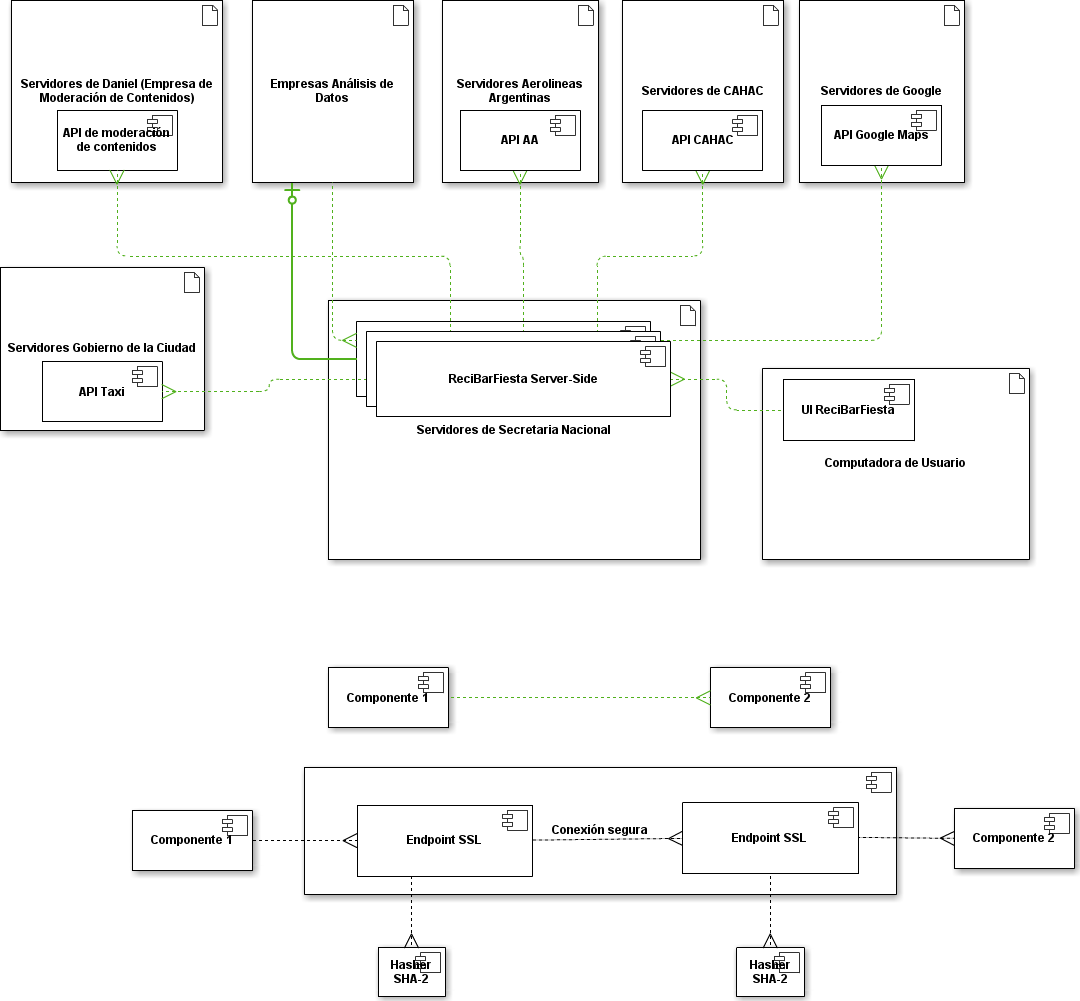
\includegraphics[width=\textwidth]{diagramas/Nivel0.png}
  \caption{\normalfont }
\end{figure} 


\subsubsection{ReciBarFiesta}

\begin{figure}[H]
  \centering
  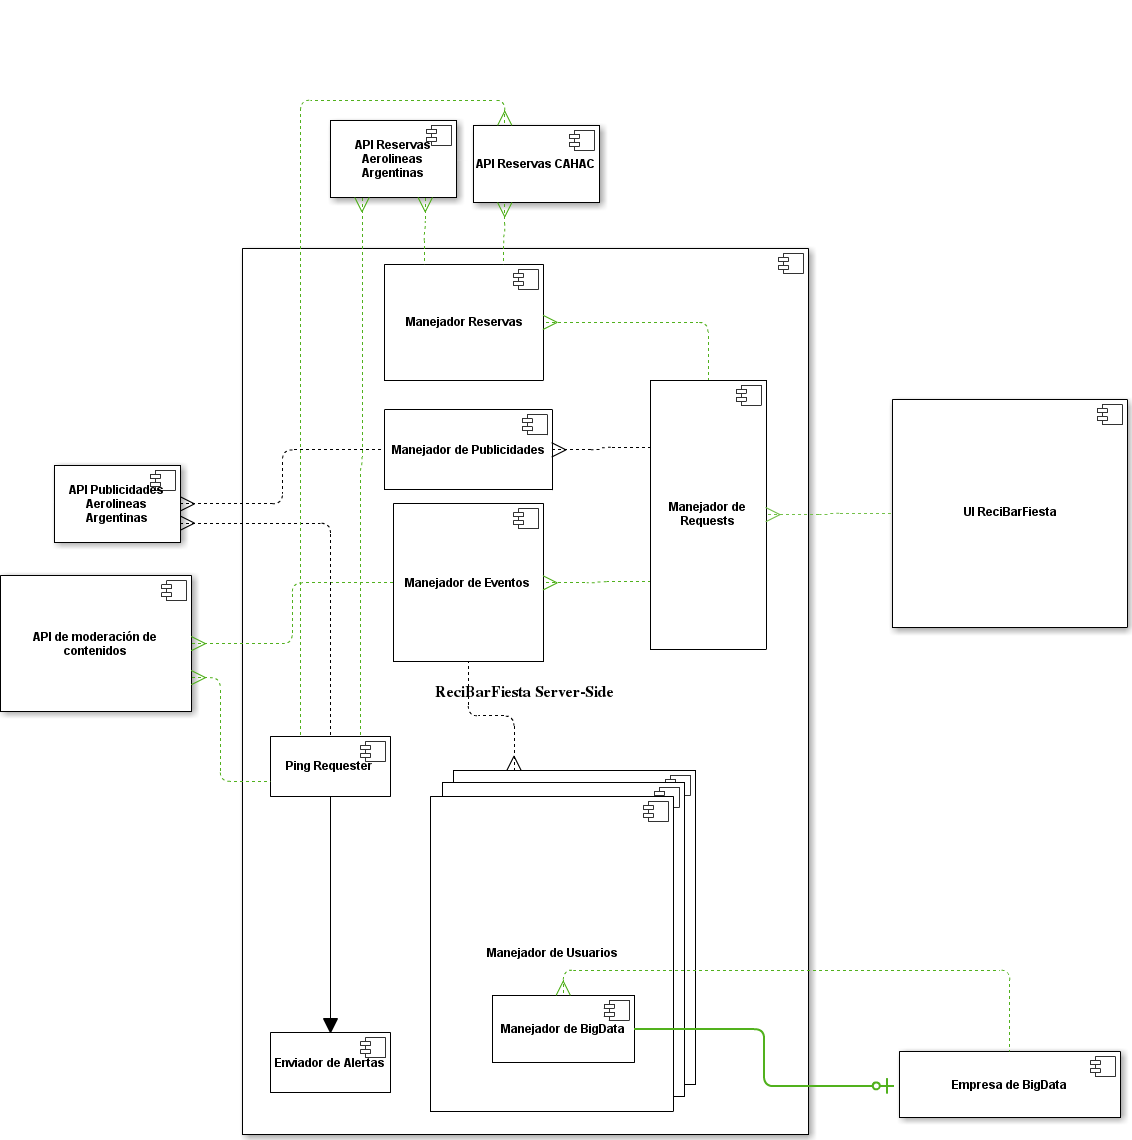
\includegraphics[width=\textwidth]{diagramas/ReciBarFiesta.png}
  \caption{\normalfont }
\end{figure} 

\subsubsection{Manejador de Eventos}

\begin{figure}[H]
  \centering
  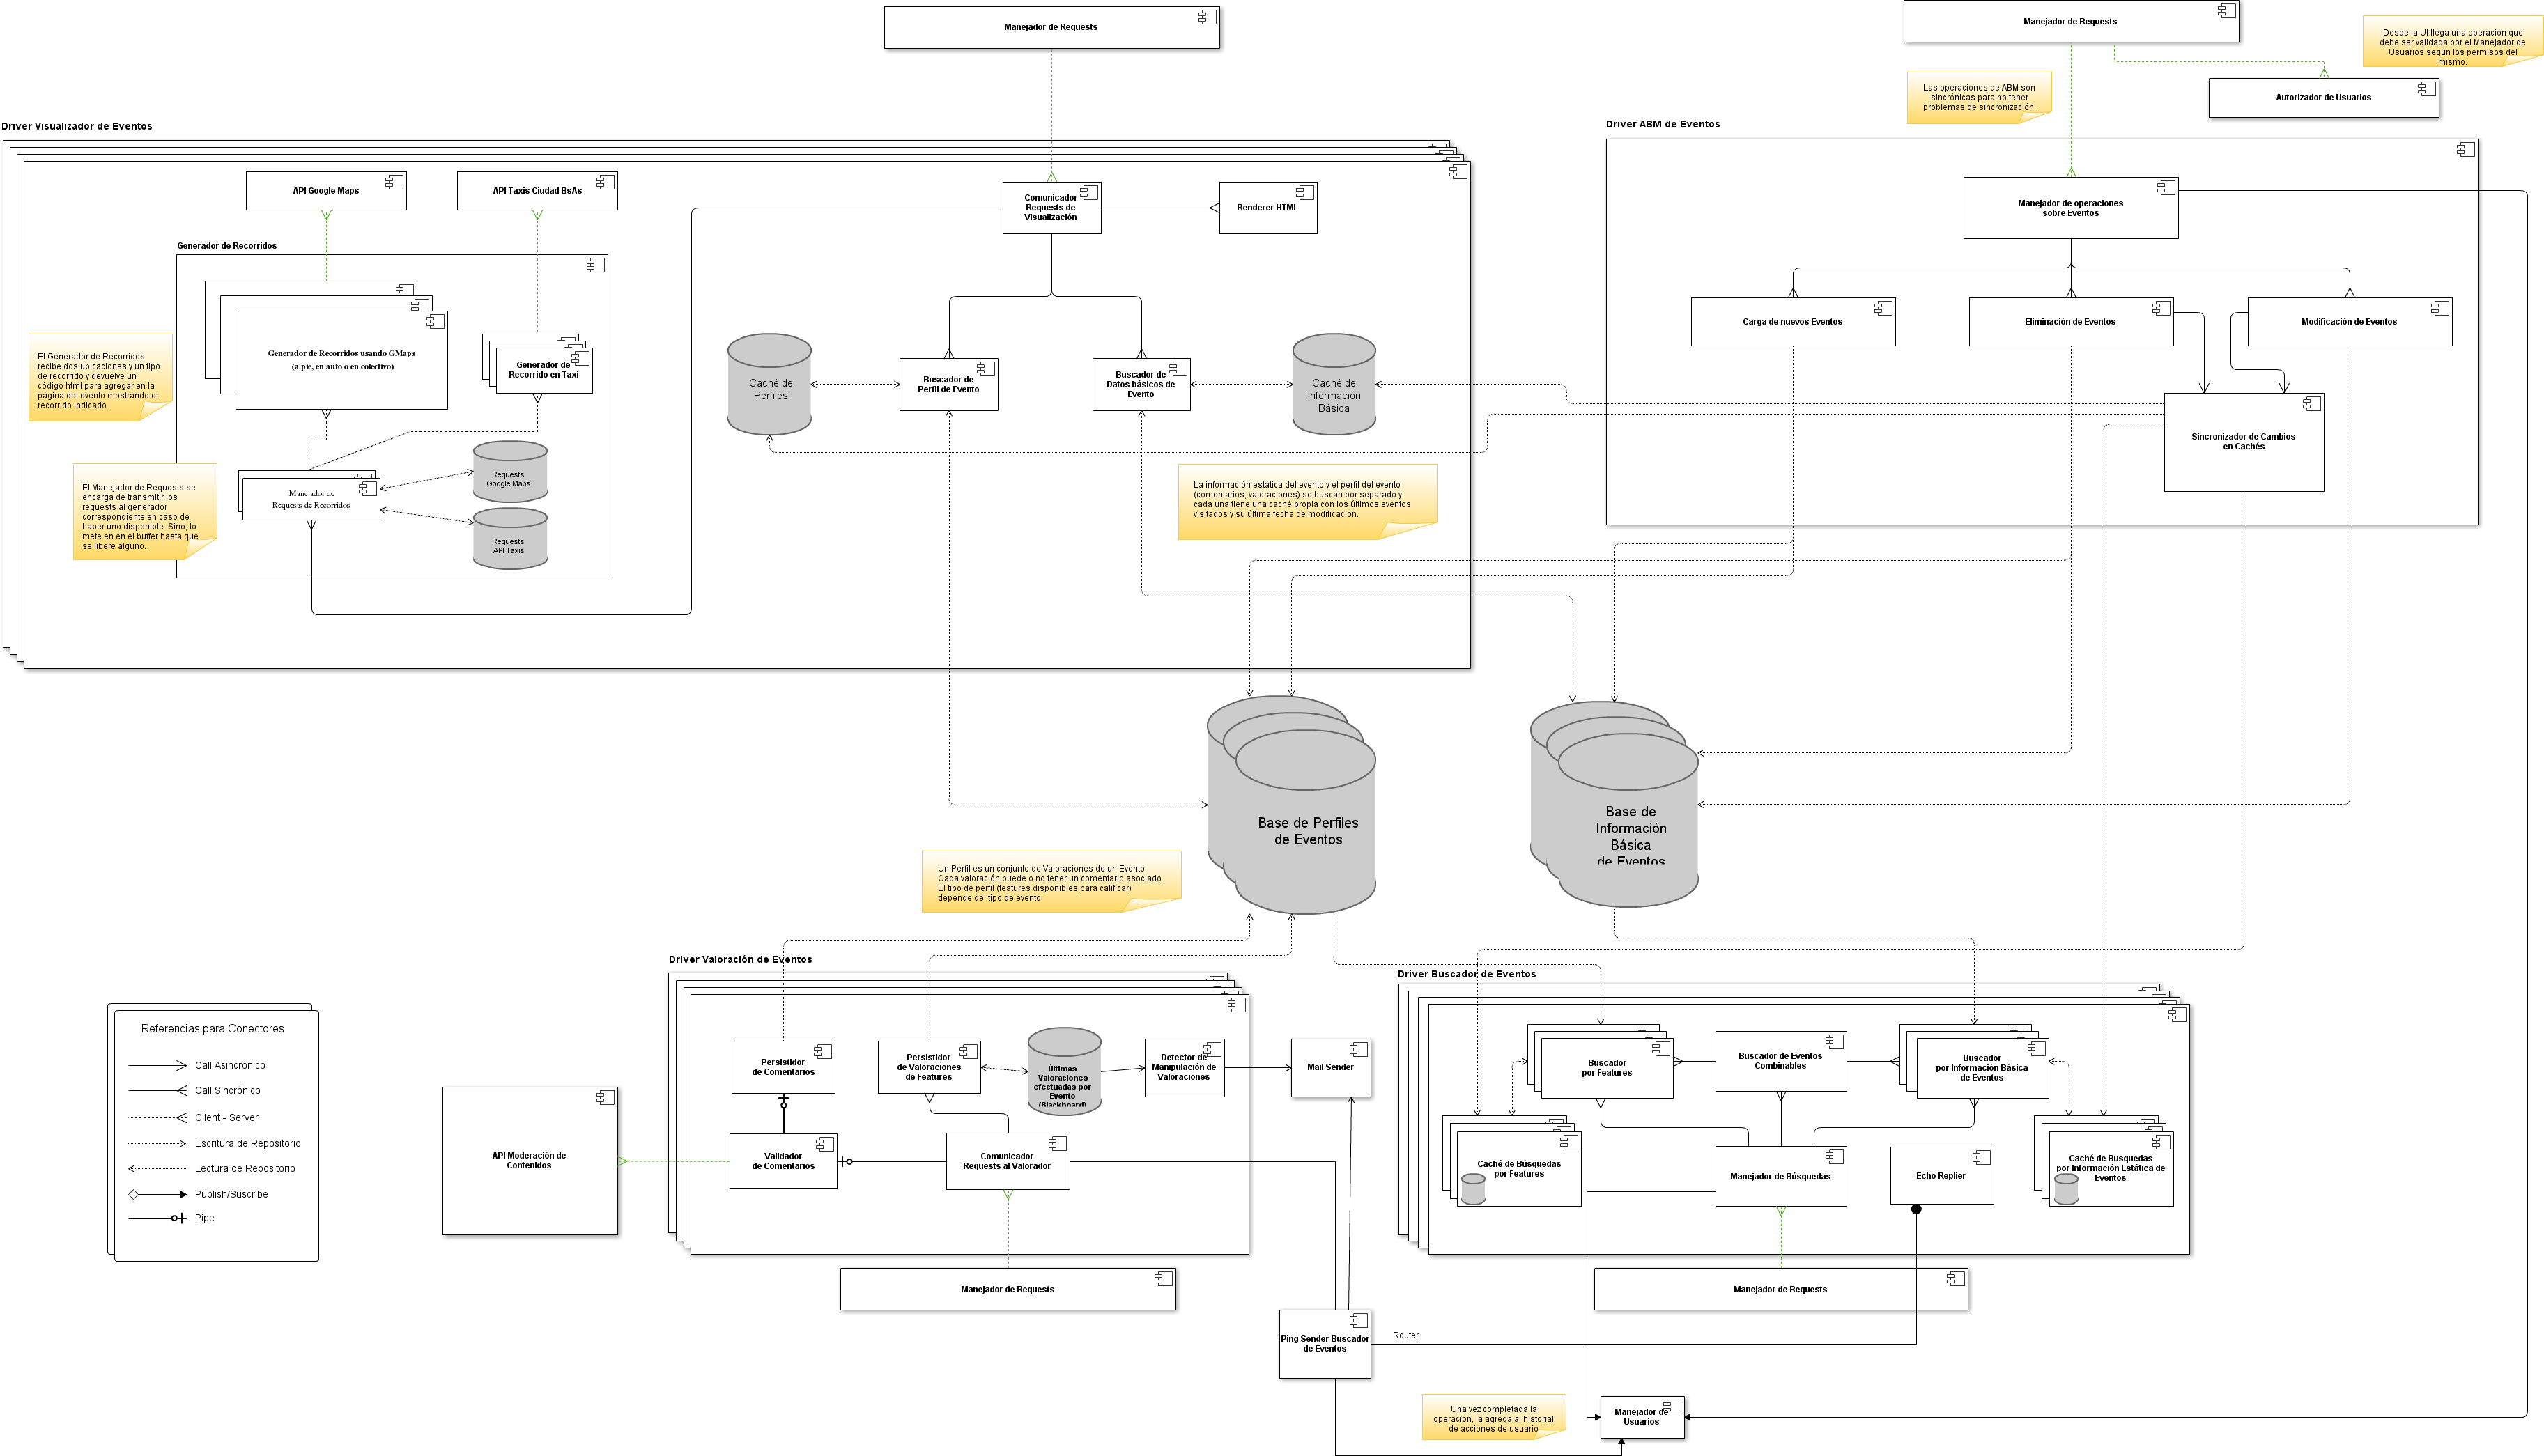
\includegraphics[width=\textwidth]{diagramas/ManejadorDeEventos.png}
  \caption{\normalfont }
\end{figure} 

\subsubsection{Manejador de Usuarios}

\begin{figure}[H]
  \centering
  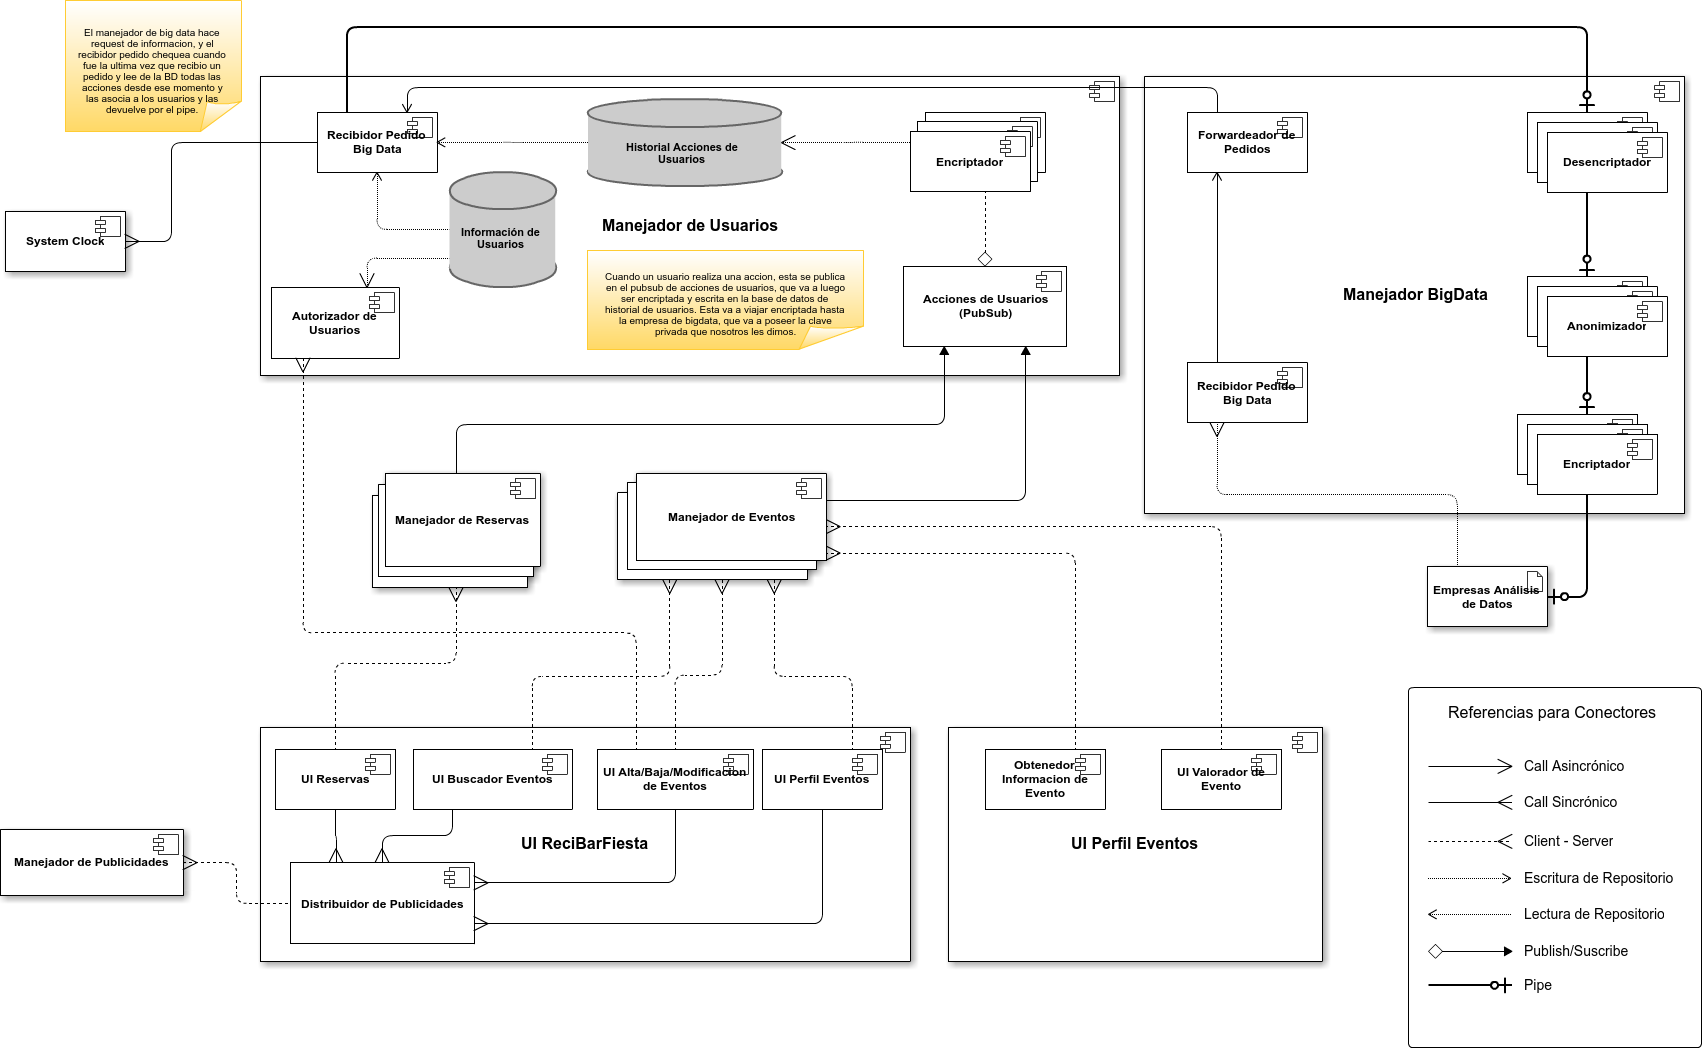
\includegraphics[width=\textwidth]{diagramas/ManejadorDeUsuarios.png}
  \caption{\normalfont }
\end{figure} 

\subsubsection{Manejador de Reservas}

\begin{figure}[H]
  \centering
  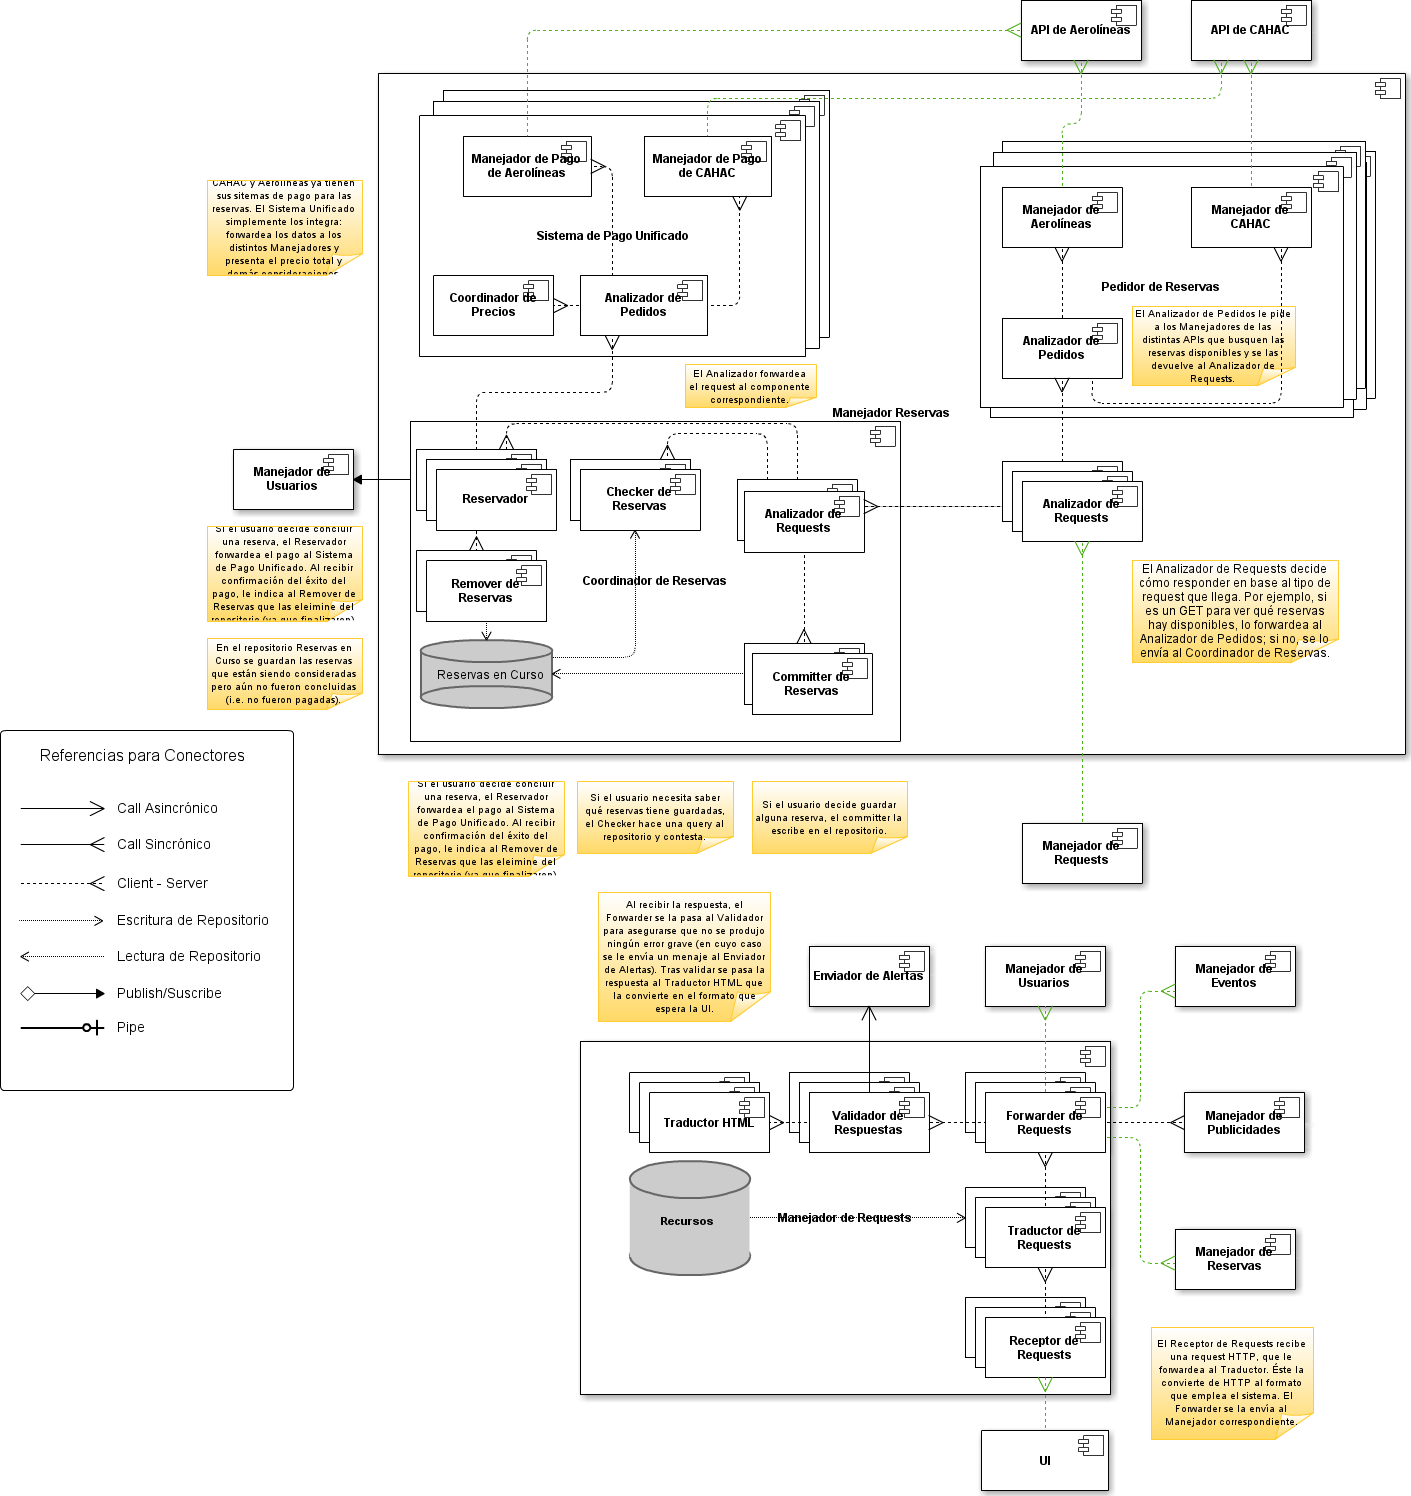
\includegraphics[width=\textwidth]{diagramas/ManejadorReservas.png}
  \caption{\normalfont }
\end{figure} 

\subsubsection{Manejador de Publicidades}

\begin{figure}[H]
  \centering
  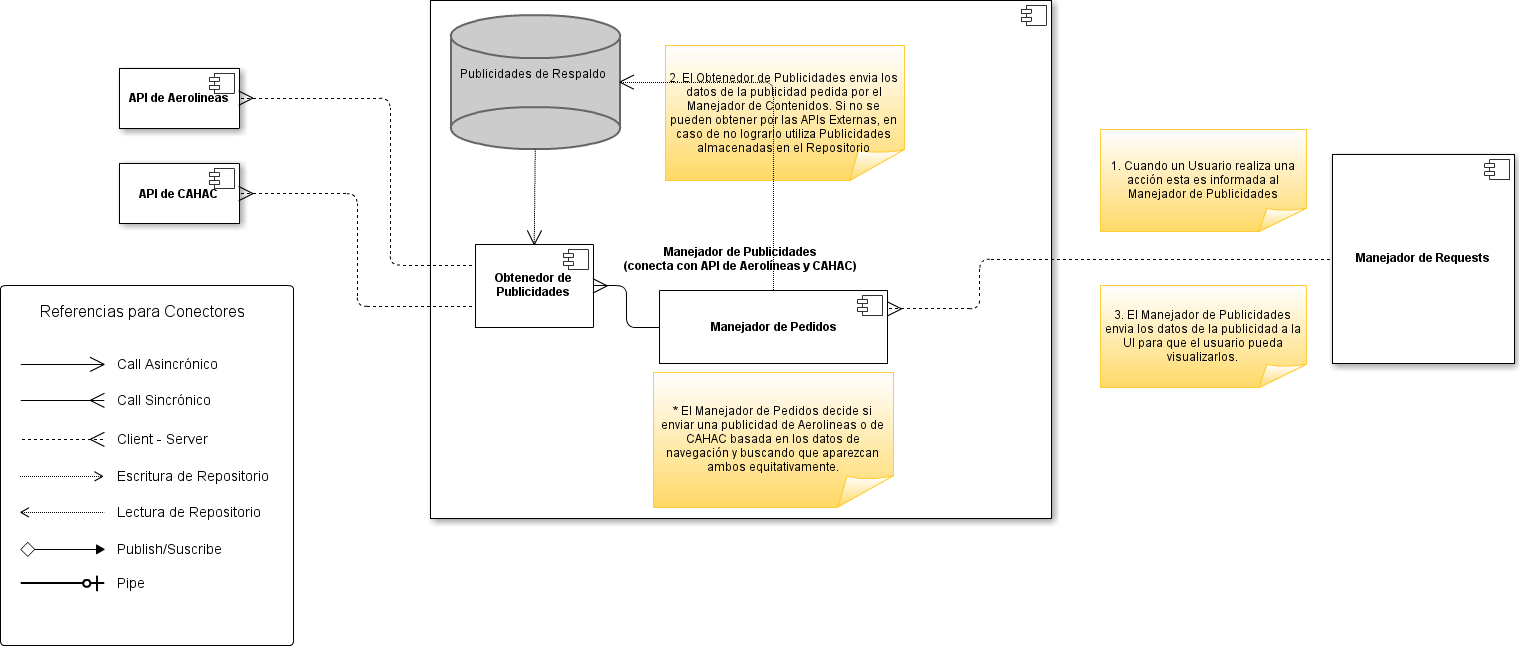
\includegraphics[width=\textwidth]{diagramas/ManejadorDePublicidades.png}
  \caption{\normalfont }
\end{figure} 

\subsection{Explicación de la Arquitectura}

\subsubsection{Manejador de Eventos}

El manejador de eventos es el encargado de responder a las distintos requests que envía un usuario de la aplicación desde la interfaz para ejecutar una acción sobre un evento: agregar uno nuevo, modificar, eliminar, valorar, visualizar y búsqueda de eventos.

Notar que los componentes de Visualización, Valoración y Búsqueda de Eventos están replicados para poder realizar muchas operaciones concurrentemente. Sin embargo, el componente de ABM no está replicado para evitar que se generen inconsistencias en la información de los eventos.

\textbf{Visualización de Eventos}

Es el encargado de obtener la información cargada en las bases de datos asociada a un evento en particular, que incluye los datos básicos del evento (así llamaremos a datos como el Nombre, Ubicación, Horario, Tipo de evento, etc.) y los datos del "Perfil del Evento" (que incluye valoraciones por cada feature según el tipo de evento y comentarios asociados a esas valoraciones realizados por los usuarios).

Supongamos que un usuario quiere acceder a la Vista de un evento en particular, al hacer click en un evento el sistema envía el ID del mismo al Manejador, en particular al componente Driver Visualizador de Eventos. Este componente recibe el request y procede a buscar la información asociada al evento (perfil y datos básicos). Para ambos casos, hay un componente encargado de realizar las consultas en la base correspondiente. Además, cada uno tiene una caché asociada con los últimos eventos visitados por los usuarios. Una vez obtenida la información, en caso de que el usuario desee ver el recorrido hasta el evento, se envía al generador de recorridos la dirección actual del usuario y la dirección del evento. Este componente se encargará de interactuar con la API necesaria: GoogleMaps en caso de que sea recorrido a pie, en auto o en colectivo, o la API de Taxis de la Ciudad, para recorridos en taxi. A través de dichas APIs generará un código HTML que se enviará al Comunicador. Luego, el Comunicador del Driver de Visualización envía toda la información al Renderer HTML para generar la página correspondiente y enviársela a la interfaz para que el usuario pueda verla.

\textbf{Alta/Baja/Modificación de Eventos}

Desde la interfaz, un usuario decide realizar una de las operaciones de ABM para algún evento en particular. Primero, el usuario debe ser autorizado por el Autorizador de Usuarios si es que tiene los permisos necesarios para realizar la operación. Una vez chequeados sus permisos, el request llega al Driver ABM de Eventos del Manejador. El Manejador de operaciones deriva el request parseado con los datos necesarios para realizar la operación al componente correspondiente: Carga de nuevos Eventos, Eliminación, o Modificación.
En caso de tratarse de Carga de un Evento, el componente chequea que el evento sea válido, y en caso afirmativo procede a agregarlo a la base de datos de Información básica y a la base de Perfiles, generando un perfil vacío.
En caso de que sea una baja de un evento, el componente elimina todas las entradas del mismo en las bases de perfiles e información básica, y luego envía un request asincrónico al Sincronizador de Cambios en Cachés, encargado de actualizar todas las cachés de los componentes del Manejador de Eventos, para que no queden con datos inconsistentes.
Por último, en caso de ser una modificación, se actualiza la información básica del evento una vez que haya sido validada, y luego se avisa al sincronizador de cachés para que ejecute las actualizaciones.
Una vez finalizada la operación, la misma se guarda en el historial de acciones por usuario.

\textbf{Valorador de Eventos}

Este componente es el encargado de almacenar las valoraciones de los usuarios en el perfil del evento correspondiente. Una valoración debe incluir al menos un valor seleccionable para los features de un evento, que dependen del tipo del mismo, y además puede o no incluir un comentario asociado a dicha valoración. El driver de valoración de eventos, en caso de que la valoración contenga un comentario, se encargará de validar el mismo interactuando con la API de moderación de contenidos. Una vez validado, procederá a guardar la valoración en la base de Perfiles del evento correspondiente. En caso de no ser validado por la API, se almacenará la valoración sin el comentario y se devolverá un mensaje de error.

\textbf{Buscador de Eventos}

El Driver Buscador de Eventos manejará las búsquedas realizadas por los usuarios, dividiéndolas en búsquedas por Features o búsquedas por Información Básica del evento. El Manejador de Búsquedas parseará el request del usuario y enviará la búsqueda al componente Buscador correspondiente según el tipo de la misma. Cada uno de estos componentes cuenta con una Caché donde se almacenarán las búsquedas más populares realizadas por los usuarios, que serán actualizadas periódicamente. Las cachés cuentan con tres niveles (primario, secundario, y terciario) según el nivel de popularidad de las búsquedas para garantizar performance. Una vez realizada la búsqueda, en caso de ser requerido por el usuario, el manejador enviará los resultados al Componente buscador de Eventos Combinables, para que genere búsquedas de eventos combinables (cercanos, temáticas relacionadas, etc.), que luego serán efectuadas por el Buscador correspondiente según se trate de búsquedas en la base de datos de perfiles o de información básica. Una vez obtenidos los resultados, se actualizan las cachés, se notifica al historial de usuario la acción realizada, y se devuelve una página con los resultados y links a las vistas de los eventos encontrados.


\subsection{Aspectos particularmente importantes y cómo los resolvimos}

\subsubsection{¿Cómo se cumplen los requerimientos de seguridad respecto de los servicios para las empresas enfocadas en los grandes datos?}

Utilizamos varias tácticas para cumplir con los requerimientos de seguridad.

Primero tenemos todos los datos de las bases de datos encriptados, tanto de la base de datos de Información de Usuarios como de Acciones de Usuarios. Esto permite que, aunque haya una intrusión en el sistema y las bases de datos se vean expuestas, el atacante no podrá obtener ningún tipo de información sobre los usuarios. Esto es una táctica de resistencia a ataques.

Otra táctica que usamos es la desanonimización de los datos de los usuarios. Esto, desde algún punto de vista, puede verse como la táctica de separación de entidades. Esto nos permite que, por ejemplo, si hay alguna intrusión del lado de la empresa de grandes datos, no se pueda recuperar la información personal de los usuarios.

Por último, todos los enlaces entre la empresa de grandes datos y nuestro sistema son a través de una conexión segura como la que está explicada en los diagramas, utilizando por ejemplo TLS, que nos brinda autenticación y no repudio, que son dos características muy deseables para el tipo de conexión que queremos establecer.

\subsubsection{¿Cómo es la interacción con los servicios externos? (API de moderación, Aerolíneas, Cámara de Hoteles) ¿Hay disponibilidad? ¿Seguridad?}

La interacción con los servicios externos es siempre mediante manejadores de esos servicios externos que nos abstraen y nos permiten reemplazarlos fácilmente.

En cuanto a disponibilidad, implementamos un Ping Requester, que cada 10 minutos envía pings a los servicios para verificar que estén disponibles y funcionando correctamente. Si no lo están, se envía un mail al on-call del equipo, reportando el problema. Esta táctica es de detección de errores, y permite disminuir el downtime.

Por otra parte, en servicios como las publicidades, implementamos caches de publicidades, que ante un problema de conexión con la API de Aerolíneas Argentinas que nos provee de publicidades, carga una publicidad de la cache de publicidades y la muestra.

En cuanto a seguridad, implementamos el conector seguro para conectarnos a todos los servicios externos. Estos conectores usan TLS, que brinda integridad, autenticación y no repudio, todo lo deseable en una conexión segura. Esto nos permite resistir muy bien a los ataques. Además, nunca se envía información personal de los usuarios. Cada vez que información de usuarios va a ser envíada fuera del sistema, es anonimizada (se le quitan los datos personales y se la deja
inidentificable a una persona física) y encriptada.

\subsubsection{¿Cómo se logra perfomance para responder las búsquedas de los usuarios?}

La performance se logra utilizando variadas tácticas.

La táctica más simple es la de replicación. Tenemos nuestro servidor replicado y tenemos un manejador de requests entre la UI y el server side, que actúa como distribuidor de requests y balanceador de carga.

Además, dentro del Manejador de Eventos, en la sección que concierne a la búsqueda de eventos, tenemos múltiples caches que permiten obtener la información a muchisima más velocidad que haciendo la búsqueda de cero. 

Además, tenemos replicadas nuestras bases de datos, lo cual permite atender varias requests de lectura al mismo tiempo sin problemas.



\newpage

\section{Conclusión}
\subsection{Métodos usados (UP vs. Ágil)}

UP y los métodos ágiles (como Scrum, que usamos para el primer TP) son iterativos incrementales. Sin embargo tienen varias diferencias.

UP se centra en la arquitectura, y facilita su refinamiento progresivo.

En el primer TP teníamos tres artefactos que guíaban el desarrollo de software: un Product Backlog, un Sprint Backlog y un Burndown Chart. Un backlog es simplemente una lista de prioridad de cosas a hacer. El Burndown Chart sirve para graficar el progreso durante la iteración actual. Estas tres herramientas son lo que se usa para planificar y hacer el seguimiento del proyecto en Scrum.

UP, por otro lado, contiene una larga lista de documentos y herramientas para planificar el proyecto. Por ejemplo, una planificación de una iteración de UP es muchísimo más detallada que para Scrum, dado que incluye riesgos, tareas, recursos asignados a tareas y dependencias entre tareas.


\begin{figure}[H]
  \centering
  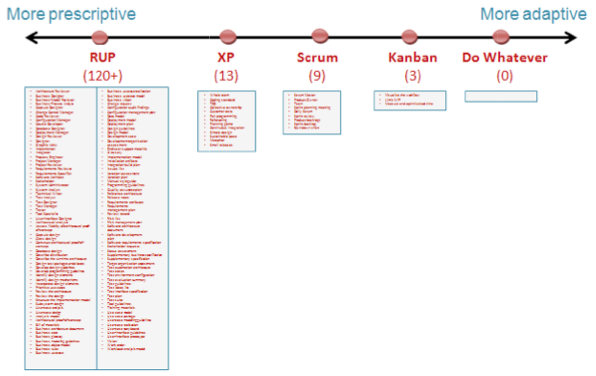
\includegraphics[width=0.7\textwidth]{img/up-agile.png}
  \caption{\normalfont Comparación de varias metodologías de desarrollo.}
\end{figure} 

\subsection{Programming in the small y Programming in the large}

Programming in the large y programming in the small describen dos aproximaciones diferentes al diseño y desarrollo de software. 

Programming in the large involucra en general productos de software desarrolloados por grupos a lo largo de extensas cantidades de tiempo. Con programming in the large, los diseñadores hacen hincapié en particionar el trabajo en modulos con interacciones bien definidas. Esto requiere una cuidadosa planificación además de una cuidadosa documentación. Programming in the large en general se refiere a diseñar el sistema desde un alto nivel, donde solo importa el estado de los módulos y sus interacciones, y no su implementación real.

Debido a todas estas características, el programming in the large es importante planificar a largo plazo, tener en cuenta riesgos y darle mucha importancia a la arquitectura del software. Por esta razón, programming in the large suele estar asociado con UP.

Por otro lado, programming in the small describe la actividad de escribir pequeños programas, es decir, cuyo desarrollo toma poco tiempo. En general programming in the small es llevado a cabo por personas individuales o pequeños equipos.

Debido a que en general se busca velocidad en el desarrollo de estas pequeñas piezas de software, y mejorarlas de manera incremental, programming in the small suele asociarse con métodos de desarrollo ágiles, como Scrum.

\subsection{Conclusiones generales}

Como conclusión general, podemos decir que los dos trabajos prácticos nos permitieron apreciar dos m\'etodos de desarrollo y planificación de desarrollo de software muy distintos, que aplican a situaciones distintas. 

UP permite llevar a cabo proyectos enormes, que se extenderán durante mucho tiempo. Por eso se requiere planificar todo al detalle, pensar en los riesgos, diseñar la arquitectura del software puntillosamente, de tal manera que la gran inversión de tiempo y dinero no sea en vano.

Por otro lado, las metodologías ágiles que vimos para el primer trabajo práctico, permiten desarrollar de forma muy rápida softwares pequeños. Es muy buena para desarrollar prototipos o borradores de softare (por ejemplo, Most Viable Products), y luego incrementarlos de a poco. Sin embargo, los equipos tienen que ser más pequeños que para UP (que por su alto nivel de planeamiento soporta equipos muchísimo más grandes).

\newpage

\section{Referencias}

\end{document}
